\chapter[Introduction]%
{Introduction}

\section{The occurrence of ferroptosis}

Ferroptosis is a complex process with many contributing, interconnected factors. At its core, it is an intracellular iron-dependent form of cell death that is distinct from apoptosis, necrosis, and autophagy \parencite{ferro_cd}. As the name suggests, this phenomenon is principally driven by iron molecules absorbed by cells from the surrounding extracellular environment. One such receptor is transferrin receptor 1 (TFR1), which mediates endocytosis of diferric transferrin \citep{tfr1}. This intracellular iron is often transported and stored in storage proteins such as ferritin, aiding in maintaining iron homeostasis and metabolism \citep{ferritin}.

Labile iron, however, which refers to loosely bound or chelatable iron, becomes a critical player in the ferroptotic process. Labile iron participates in the Fenton reaction, leading to the generation of reactive oxygen species (ROS), particularly hydroxyl radicals \citep{labile_iron}. ROS, in turn, contributes to oxidative stress within the cell. 

Polyunsaturated fatty acids in cellular membranes are highly susceptible to oxidative damage by ROS \citep{lpperox}. Lipid peroxides are formed as a result of the oxidation of these fatty acids. Accumulation of lipid peroxides disrupts the integrity of cellular membranes, particularly the lipid bilayer \citep{lppmembrane}. Membrane damage leads to the loss of compartmentalization and function within the cell, including the mitochondrion \citep{lppmito}.

Healthy mammalian cells stave off this threat in a number of ways. The primary cellular mechanism of protection against oxytosis/ferroptosis is mediated by glutathione peroxidase 4 (GPX4), a glutathione-dependent hydroperoxidase that converts lipid peroxides into non-toxic lipid alcohols \citep{gpx4}. Glutathione itself, which is produced from cysteine, is able to neutralize ROS present within the cell directly, playing the role of antioxidant \citep{glutath}. 

Even when glutathione peroxidase functionality is uncompromised, research has shown that the mitochondrion plays a substantial role in ferroptosis regulation and induction, being the major compartment for cellular iron metabolism \citep{mito_ferro2}. Mitochondrial shrinkage and rupture are also common observations when a cell undergoes ferroptosis, since this organel is enveloped in a membrane \citep{mito_ferro}.

\begin{figure}[ht]
        \begin{center}
            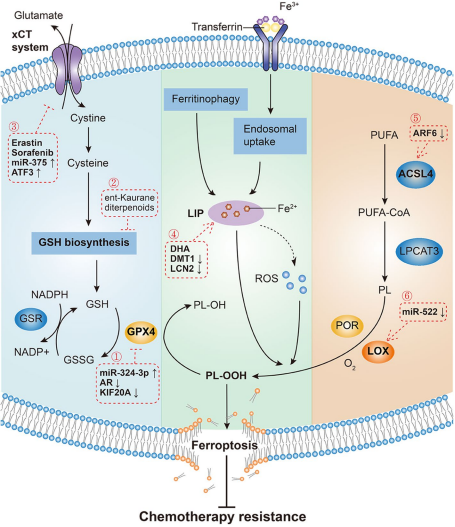
\includegraphics[width = 0.5\textwidth]{Fig/ferroptosis.png}
        \end{center}
        \caption{Figure depicting the various regulatory pathways associated with ferroptosis \citep{ferro_cancer}.}\label{fig:ferro_mech}
\end{figure}

\section{Ferroptosis in cancer therapy}

Cancer is the second leading cause of death worldwide, behind cardiovascular disease \citep{cancer}. However, improvements in cancer survival rates due to the use of precision medicine or immunotherapy 

There are a number of ways to counteract this resistance, including inhibition of glutathione synthesis, overexpression of transferrin receptors, underexpression of or defective ferritin (including the chaperone proteins that fill the ferritin) and/or ferroportin proteins (which export labile iron bound to chaperones outside the cell) \citep{ferro_drugs}.

\section{Oxford Nanopore Episequencing}

Nanopore sequencing is a next-generation sequencing technology that enables the real-time analysis of DNA or RNA molecules as they pass through a nanoscale pore. This technique is based on the principle that as a DNA strand translocates through a nanopore, changes in the electrical current can be measured and used to deduce the sequence of the DNA molecule \cite{ont}. The raw electrical signal is translated into DNA sequence information through a process called basecalling. DNA methylation involves the addition of a methyl group to a cytosine base (5-methylcytosine). Nanopore sequencing can detect these modifications as changes in the electrical current during translocation using specialized algorithms and basecallers. One of the key advantages of nanopore sequencing is its ability to generate long reads, providing information about entire genomic regions in a single continuous sequence.

Adaptive sampling is a feature associated with PromethION that helps optimize the sequencing process by adjusting data collection parameters in real-time based on the characteristics of the DNA being sequenced. The system monitors various parameters such as the quality of the signal, the speed at which the DNA is translocating through the nanopore, and other relevant metrics \citep{ont_as}. The software requires a user to upload a file of whitelisted reference sequences, and the system can be set to either deplete or enrich for these on a specified set of channels. 

In order to achieve this, the software basecalls the first few hundred bases of each read and compares it with the target reference sequences. Matching or unmatching sequences are rejected, depending on whether the software is set to enrich or deplete. By using this, coverage of our genes of interest is enriched, greatly reducing noise.